% Introduction

% Problem:
% - Problem and analysis:
% - System diagram (what we want to build):
% Daniel has already made a nice diagram of this

% Robot control: (maybe after pathfinding?)
% Theory:
% - functionality
% - step/control sequence
% Implementation: (programming)
% - programming/framework etc.

% Map handling:
% Theory (how we did and thoughts):
% - Introduction (what is map handling about, what have we covered here, problems we want to solve)
% - Analysis of map input6
% - Converting analog map to digital map (intro)
% - 
% Implementation:
% - Read, compare, update 

% read google docs

% I can use \subsection and \subsubsection :)

\chapter{Map Handling}
\label{ch:map} % chapter label
The rescue robot should be able follow a given path from start to finish, based on a predefined map.
A map provides useful information about whether areas of the map are accessible or not. This is an important element in path-finding.
Map data can be given to the robot prior to its physical presence at a location. Once the robot is at the starting point, it has to rely on its sensors for updated information about the surroundings.

A structured way of storing the required map data for different maps was designed. 
The goal was to not only make it readable by the microcontroller,
but also allow easy user input.

%Existing pathfinding algorithms such as Dijkstra and A* was studied, 
%in order to understand what input data such algorithms typically would require. 
%The pathfinding algorihtm implemented in this project is further described in chapter \ref{ch:path}.

\newpage
\section{Map requirements}
\label{ch:map_requirements}
Maps can be found in a lot of different styles,
varying in how they represent specific informations.
Those styles often depend on the purpose of the map.

Figure \ref{sub:orient} shows a map for casual orientation purposes,
while \ref{sub:evac} shows a standardized evacuation plan.

\begin{figure}[h!tp]
    \centering
    \subfloat[Section of AAU Esbjerg]{%
        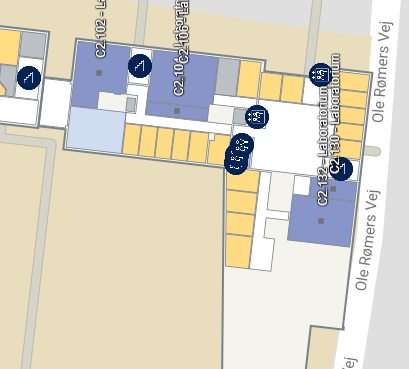
\includegraphics[width=0.4\textwidth]{figures/map/floorplan_aau.png}%
        \label{sub:orient}
        }%
    \hspace{0.1\textwidth}
    \subfloat[School layout example]{%
        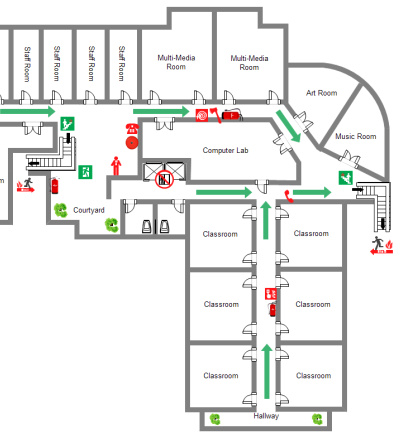
\includegraphics[width=0.4\textwidth]{figures/map/floorplan_school.png}%
        \label{sub:evac}
        }%
    \caption{Examples of different maps}
    \label{fig:floor_plans}
\end{figure}
% https://www.edrawsoft.com/school-layout-example.php

Such maps are often very visual, providing a lot of detailed information to the reader.
The way the information is represented differently,
makes it very hard to be interpreted automatically.

A map must provide necessary information,
in a way that can be interpreted by the micro controller.
For this project we decided that a simplified map, would be sufficient.

Table \ref{table:map_data} shows the data the map should include,
as well as some areas that have been delimited from.

\begin{table}[h!]
	\centering
	\caption{Map data}
	\begin{tabular}{|p{0.4\textwidth}||p{0.4\textwidth}|}
		\hline
		Data to be included & Data to delimit from \\ 
		\hline
		Map dimensions 		& \parbox[t]{0.4\textwidth}{Differences in height\\(levels, stairs etc.)}\\
		\hline
		Start position 		& Door openings \\
		\hline
		Finish position 	& \parbox[t]{0.4\textwidth}{Ground surface\\(slipping, traction)} \\
		\hline
		Walls 				& Objects\\
		\hline
	\end{tabular}
	\label{table:map_data}
\end{table}


\section{Map coordinates}
\label{sec:map_coordinates} % section label

\begin{figure}[h!tp]
    \centering
    \subfloat[Section of AAU Esbjerg]{%
        \includegraphics[width=0.4\textwidth]{figures/map/2d-map-coordinates.png}%
        \label{sub:orient}
        }%
    \hspace{0.1\textwidth}
    \subfloat[School layout example]{%
        \includegraphics[width=0.4\textwidth]{figures/map/2d-map-array.png}%
        \label{sub:evac}
        }%
    \caption{Examples of different maps}
    \label{fig:floor_plans}
\end{figure}
%https://i.stack.imgur.com/tFdLk.gif

\section{Map design}
\label{sec:map_design} % section label
Show the map + wiki\\
Explain we made the map size dynamic to handle any map size
Explain how to store wall as hex value?\\
\\
\begin{figure}[htp]
    \centering
    \subfloat[ASCII]{%
        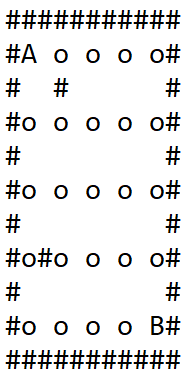
\includegraphics[resolution=96]{figures/map/5x5map_ascii.png}%
    }
    \hspace{0.2\textwidth}
    \subfloat[UTF8]{%
        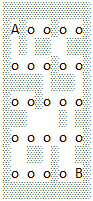
\includegraphics[resolution=96]{figures/map/5x5map_utf8.png}%
    }
    \caption{5x5 map}
    \label{fig:5x5map}
\end{figure}

\section{Check map}
\label{sec:map_check} % section label
Remember we have a chapter dedicated to scan.\linebreak
Based on scenario things might have dramatically changed, even to the point of map being useless. Explain how map is updated.

\section{Implementation}
\label{sec:map} % section label
Code here, or parts of code under each section?\\
\\
Like with many others,
is the first step in Dijkstra's algorithm to reduce the map to the necessary minimum.
After this reduction, the map only consists of \emph{nodes} and \emph{edges}.
An edge connects two nodes together and has one integer \emph{travel cost}.
In this integer is stored how much it costs to traverse along that edge,
measured in the metric that should get optimized (in our case distance).


